\section{Theorie}
\label{sec:Theorie}

Ziel des Versuches ist es, die Kenngrößen der Wärmepumpe zu 
ermitteln, indem der Transport von Wärmeenergie zwischen
zwei Wärmereservoiren untersucht wird.

\subsection{Das Prinzip der Wärmepumpe}

Ohne äußere Einflüsse findet Temperaturänderung in Form von Wärmeabgabe
vom heißeren zum kälteren Körper oder Medium statt. Durch aufgewandte 
(mechanische) Arbeit $A$ kann dieser Prozess jedoch auch in anderer
Richtung ablaufen. 

Gemäß dem ersten Hauptsatz der Thermodynamik beträgt 
die an das wärmere Medium abgegebene Wärmemenge $Q_1$, die von dem kühleren 
Medium aufgenommene Wärmemenge $Q_2$ zuzüglich der Arbeit $A$. Dementsprechend gilt

\begin{equation}
    Q_1 = Q_2 + A
    \label{eqn:Wärm}
\end{equation}

Die Güteziffer $\nu$ der Wärmepumpe gibt dabei das Verhältnis der abgegebenen 
Wärmemenge $Q_1$ zur aufgewandten Arbeit $A$ an

\begin{equation}
    \nu = \frac{Q_1}{A}
    \label{eqn:Güte}
\end{equation}

Der zweite Hauptsatz der Thermodynamik führt für die reduzierten Wärmemengen 
zu der Beziehung, dass deren Summe $\int \frac{\symup{d}Q}{T}$ null beträgt. 
Aus dieser folgt

\begin{equation}
    \frac{Q_1}{T_1} - \frac{Q_2}{T_2} = 0
    \label{eqn:redWärm}
\end{equation}

Allerdings muss es sich für diese Beziehung um einen idealen reversiblen, d.h. 
umkehrbaren Prozess handeln. Vom Ideal abweichend, gilt für die technische 
Anwendung also die Ungleichung

\begin{equation}
    \frac{Q_1}{T_1} - \frac{Q_2}{T_2} > 0
    \label{eqn:ungWärme}
\end{equation}

Aus \ref{eqn:Wärm}  und \ref{eqn:redWärm} folgt

\begin{equation*}
    Q_1 = A + \frac{T_2}{T_1} \cdot Q_1 \; \text{,}
\end{equation*}

aus \ref{eqn:Güte}, für einen reversiblen Vorgang, die ideale Güte

\begin{equation}
    \nu_\text{id} = \frac{Q_1}{A} = \frac{T_1}{T_1 - T_2}
    \label{eqn:ideal}
\end{equation}

und aus \ref{eqn:Wärm} und \ref{eqn:ungWärme} für die Güte der realen Wärmepumpe

\begin{equation}
    \nu_\text{real} < \frac{T_1}{T_1 - T_2} \; \text{.}
    \label{eqn:real}
\end{equation}

Aus \ref{eqn:ideal} und \ref{eqn:real} ist abzulesen, dass die Wärmepumpe 
für kleine Temperaturdifferenzen $T_1 - T_2$ am effizientesten arbeitet, 
die aufgewandte Arbeit $A$ zur Wärmeübertragung also minimal ist.

\subsection{Die Arbeitsweise der Wärmepumpe}

\begin{figure}
      \centering
      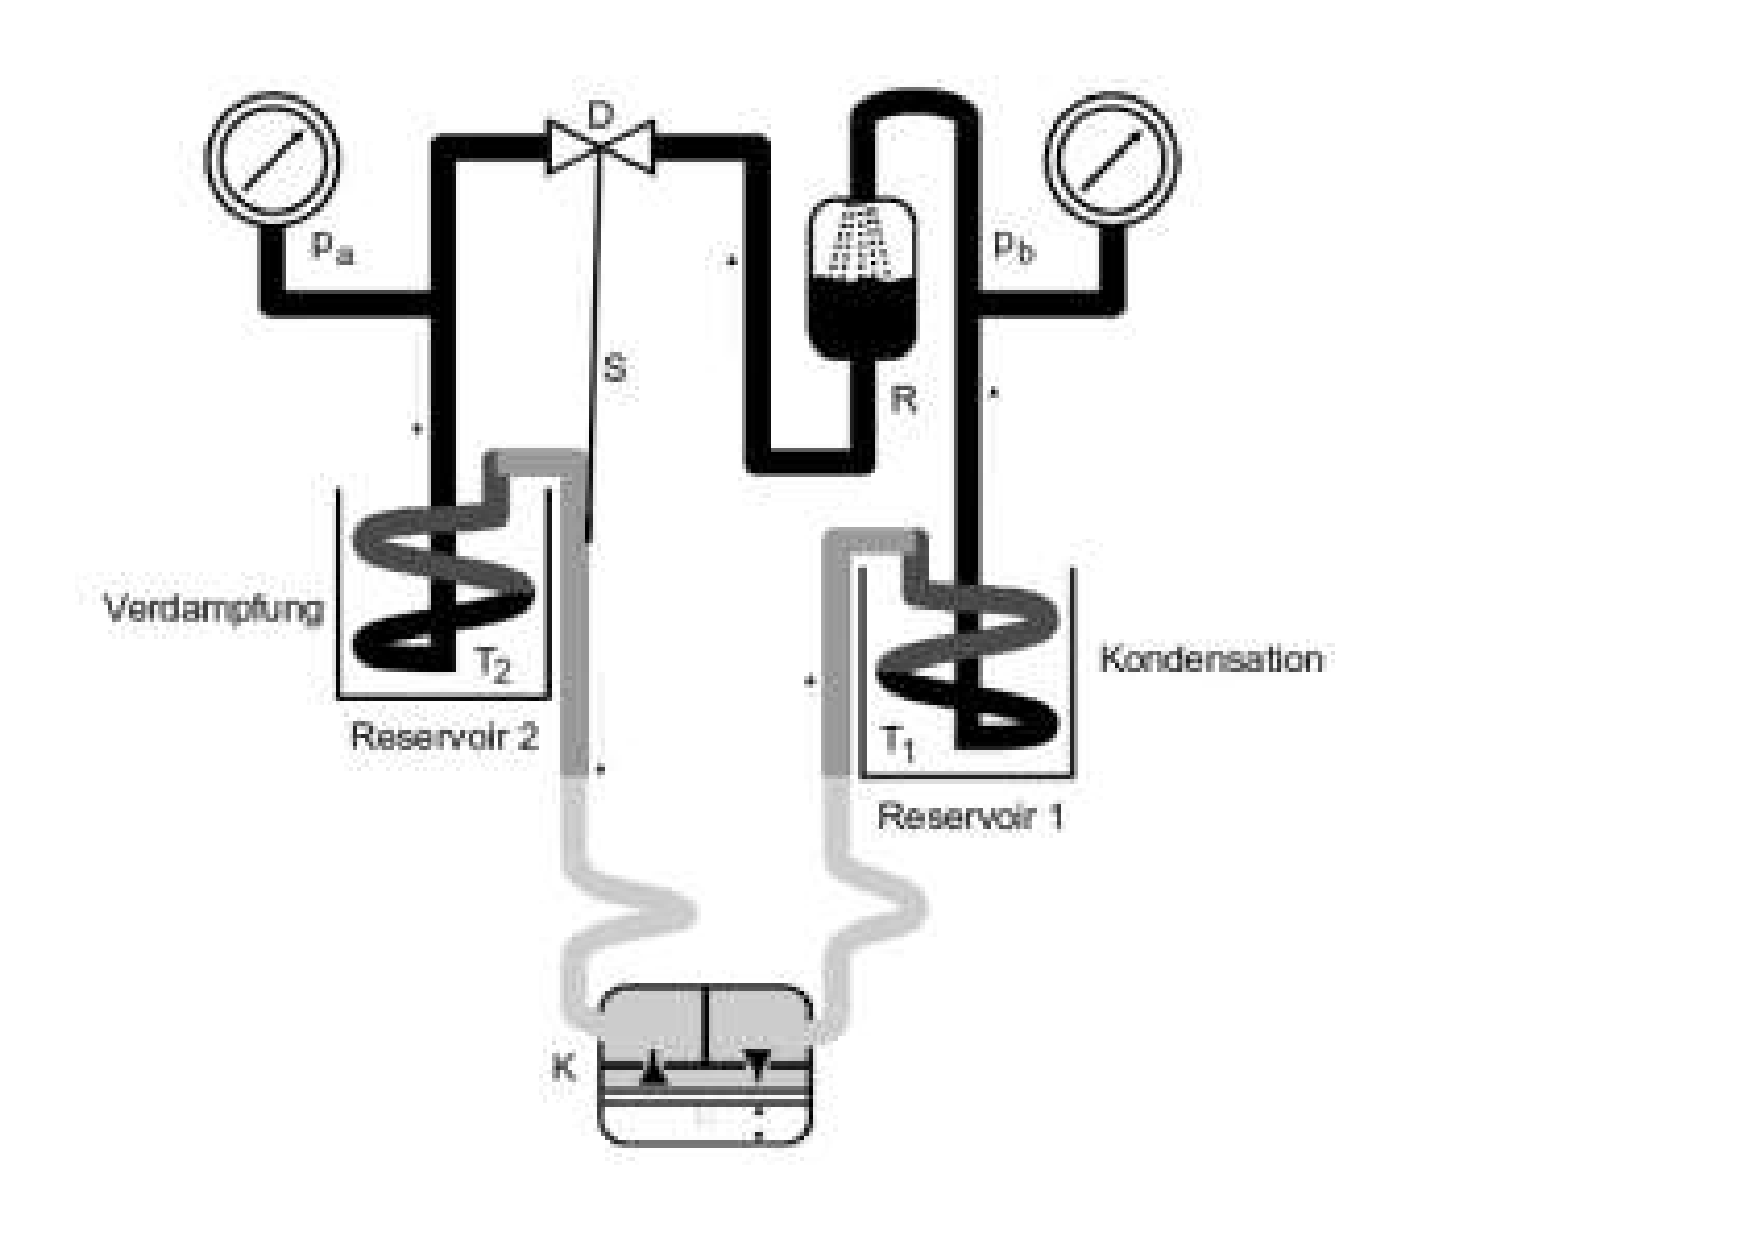
\includegraphics[scale=0.4]{aufbau2.pdf}
      \caption{Aufbau einer Wärmepumpe [1]}
      \label{fig:aufbau2}
\end{figure}

In der Wärmepumpe fungiert ein reales Gas als Transportmedium, welches 
bei Wärmeaufnahme verdampft und die Wärme durch Kondensation wieder abgibt.
Demzufolge wird die Wärmeenergie als Phasenumwandlungsenergie transportiert.
Vorteilhaft ist daher die Verwendung von Gasen hoher Kondensationswärme. 

In Abbildung \ref{fig:aufbau2} ist der Aufbau der Wärmepumpe schematisch 
dargestellt. Demnach sorgt der Kompressor K für einen Kreislauf, durch 
den das Transportgas sowohl beide Wärmereservoires, als auch ein 
Drosselventil D durchläuft. An diesem entsteht ein Druckunterschied 
$p_\text{b} - p_\text{a}$. Dabei ist das Transportgas bei Druck $p_\text{b}$ 
und Temperatur $T_1$ flüssig und bei $p_\text{a}$ und $T_2$ gasförmig.

Dem kälteren Reservoire 2 wird durch das Verdampfen des Transportgases 
die Verdampfungswärme $L$ pro gramm entzogen. Darauf wird das Gas im 
Kompressor K adiabatisch komprimiert, sodass dessen Druck und Temperatur steigen
und es schließlich die Kondensationswärme $L$ pro gramm an das Reservoire 1 abgibt.

Weitere nötige Komponenten der Wärmepumpe sind ein Reiniger R, der die Blasen 
im flüssigen Medium entfernt, sowie ein Steuerungselement S, welches mit dem 
Drosselventil D gekoppelt ist und das schädliche Eindringen flüssigen 
Mediums in den Kompressor K über Kontrolle der Temperaturdifferenz am Ein- 
und Ausgang des Reservoires 2 verhindert.

\subsection{Die Bestimmung der Kenngrößen einer realen Wärmepumpe}

\begin{figure}
    \centering
    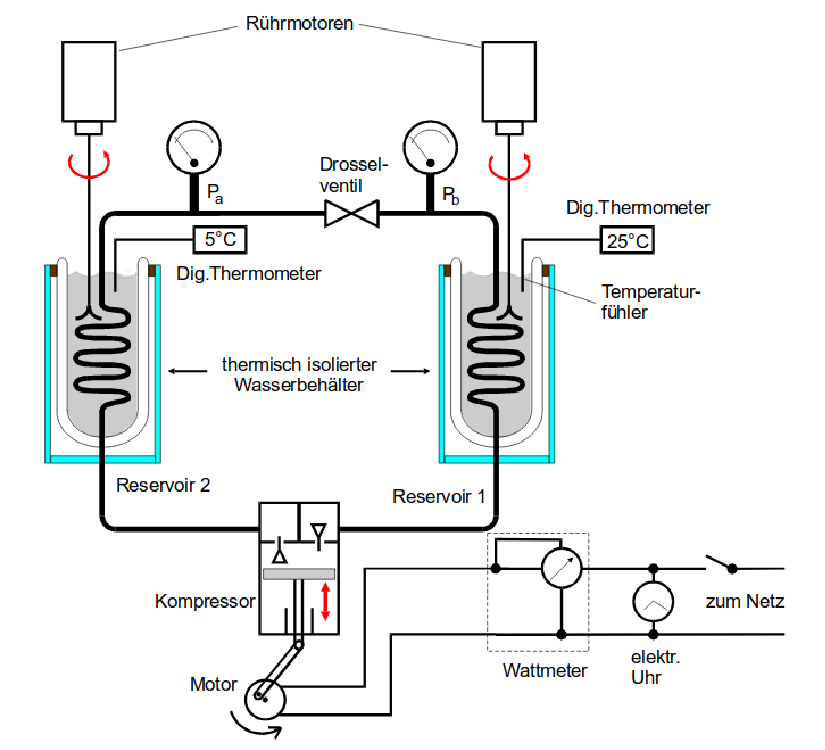
\includegraphics[scale=0.7]{aufbau.pdf}
    \caption{Aufbau der Messapparatur [1]}
    \label{fig:aufbau}
\end{figure}

Die Kenngrößen der realen Wärmepumpe sind die Güteziffer $\nu$, der 
Massendurchsatz $\frac{\symup{d}m}{\symup{d}t}$, sowie die mechanische 
Kompressorleistung $N_\text{mech}$.

Für die zeitabhängigen Messungen der Drücke $p_\text{a}$, $p_\text{b}$ 
gibt es, gemäß Abbildung \ref{fig:aufbau}, zwei jeweils zwischen dem Reservoires und dem 
Drosselventil D installierte Manometer. Für die Temperaturverläufe gibt es 
zwei digitale Thermometer in den Reservoires und für die Leistungsaufnahme
des Kompressors ein Wattmeter.

Die Reservoires befinden sich in thermisch isolierten Gefäßen und werden während
der Messung von zwei Rührmotoren umgerührt. \\

Im Folgenden können Differentialquotienten anstelle von Differenzenquotienten 
verwendet werden, da sich die Messreihen der Temperaturen als einfache, zeitabhängige
Funktionen beschreiben lassen.

\subsubsection{Die reale Güteziffer}


Mit der Messung der Zeit $T_1$ in Abhängigkeit von der Zeit $t$ lässt sich die
reale Güteziffer als

\begin{equation}
\nu = (m_1 c_\text{w} + m_\text{k} c_\text{k})\cdot 
\frac{\symup{d} T_1}{\symup{d} t} \cdot \frac{1}{N}
\label{eqn:Güteziffer}
\end{equation}

bestimmen. 

Dabei beschreibt $m_1$ die Wassermasse und $c_text{w}$ deren 
Wärmekapazität. $m_text{k}$ beschreibt die Masse der Kupferschlange und 
des Eimers und $c_text{k}$ deren Wärmekapazität.
$N$ gibt die am Wattmeter abgelesene, über das Zeitintervall $\increment t$
gemittelte Leistungsaufnahme des Kompressors an.

\subsubsection{Der Massendurchsatz}

Mithilfe der zeitabhängigen Messung der Temperatur $T_2$ lässt sich, bei 
bekannter Verdampfungswärme $L$, der Massendurchsatz durch

\begin{equation}
\frac{\symup{d} m}{\symup{d}t} = (m_2 c_\text{w} + m_\text{k} c_\text{k}) \cdot 
\frac{\symup{d} T_2}{\symup{d}t} \cdot  \frac{1}{L}
\label{eqn:Massendurchsatz}
\end{equation}

bestimmen.

Fast analog zur vorherigen Bestimmung der Güteziffer wird nun die Wassermasse
$m_2$ des Reservoires 2 benötigt.

Zur Bestimmung des Massendurchsatzes wird außerdem die Verdampfungswärme $L$
benötigt. Diese kann mit Hilfe der Clausius-Clapeyron'schen Gleichung 
berechnet werden, welche den Verlauf der Siedepunkte eines Stoffes beschreibt. 
Diese lautet: 

\begin{equation*}
\frac{\symup{d}p}{\symup{d}T} = \frac{L}{\symup{\Delta} V_m T}
\end{equation*}

Dabei ist $p$ der Dampfdruck, $T$ die Temperatur und $V_m$ die Änderung 
des molaren Volumens zwischen gasförmiger und flüssiger Phase. $\symup{\Delta} V_m$
kann dabei als molares Volumen der gasförmigen Phase genährt werden. 
Außerdem wird ein ideales Gas angenommen und dass L unabhängig von Druck 
und Temperatur ist. Dies führt zu der vereinfachten Gleichung:

\begin{equation*}
\frac{1}{p}\symup{d}p = \frac{L}{R\cdot T²}\symup{d}T.
\end{equation*}

Aufintegriert ergibt sich der Zusammenhang, aus dem $L$ bestimmt werden 
kann: 

\begin{equation}
ln(p)=\frac{L}{R}\cdot\frac{1}{T}+const.
\label{eqn:Verdampfung2}
\end{equation}

\subsubsection{Die mechanische Kompressorleistung}

Bei der Komprimierung eines Gasvolumens $V_\text{a}$ zu dem Volumen $V_\text{b}$ 
verrichtet der Kompressor die Arbeit

\begin{equation}
    A = - \int^{V_\text{b}}_{V_\text{a}} p \; \symup{d}V \; \; \text{.}
\end{equation}

Für eine adiabatische Komprimierung gilt die Poissonsche Gleichung

\begin{equation}
    p_\text{a} V^\kappa_\text{a} = p_\text{b} V^\kappa_\text{b} = p V^\kappa \; \;
    \text{,}
\end{equation}

sodass für $A$ 

\begin{equation}
    \begin{split}
        A &= - p_\text{a} V^\kappa_\text{a} \int^{V_\text{b}}_{V_\text{a}} V^{-\kappa}
        \; \symup{d}V = \frac{1}{\kappa - 1} p_\text{a} V^\kappa_\text{a} \left(
        V^{-\kappa + 1}_\text{b} - V^{-\kappa + 1}_\text{a} \right) \\
        &= \frac{1}{\kappa - 1} \left(p_\text{b} \sqrt[\kappa]{
        \frac{p_\text{a}}{p_\text{b}}} - p_\text{a}\right) V_\text{a}
    \end{split}
\end{equation}

folgt und für die mechanische Kompressionsleistung

\begin{equation}
    \begin{split}
        N_\text{mech} &= \frac{\symup{d}A}{\symup{d}t} = \frac{1}{\kappa - 1}
        \left(p_\text{b} \sqrt[\kappa]{ \frac{p_\text{a}}{p_\text{b}}} 
        - p_\text{a} \right) \frac{\symup{d}V_\text{a}}{\symup{d}t} \\
        &= \frac{1}{\kappa - 1} \left(p_\text{b} \sqrt[\kappa]{ 
        \frac{p_\text{a}}{p_\text{b}}} - p_\text{a}\right) \frac{1}{\rho}
        \frac{\symup{d}m}{\symup{d}t}
        \label{eqn:Kompressor}
    \end{split}
\end{equation}

mit Dichte $\rho$ des Transportmediums unter  dem Druck $p_\text{a}$, die sich
mit der idealen Gasgleichung unter den Normalbedingungen $p = \SI{1}{\bar}$ und
$T = \SI{0}{\celsius}$ bestimmen lässt.


